\documentclass{standalone}
\usepackage{tikz}
\usetikzlibrary{patterns, positioning}
\usepackage[sfdefault]{ClearSans} %% option 'sfdefault' activates Clear Sans as the default text font
\usepackage[T1]{fontenc}

\begin{document}
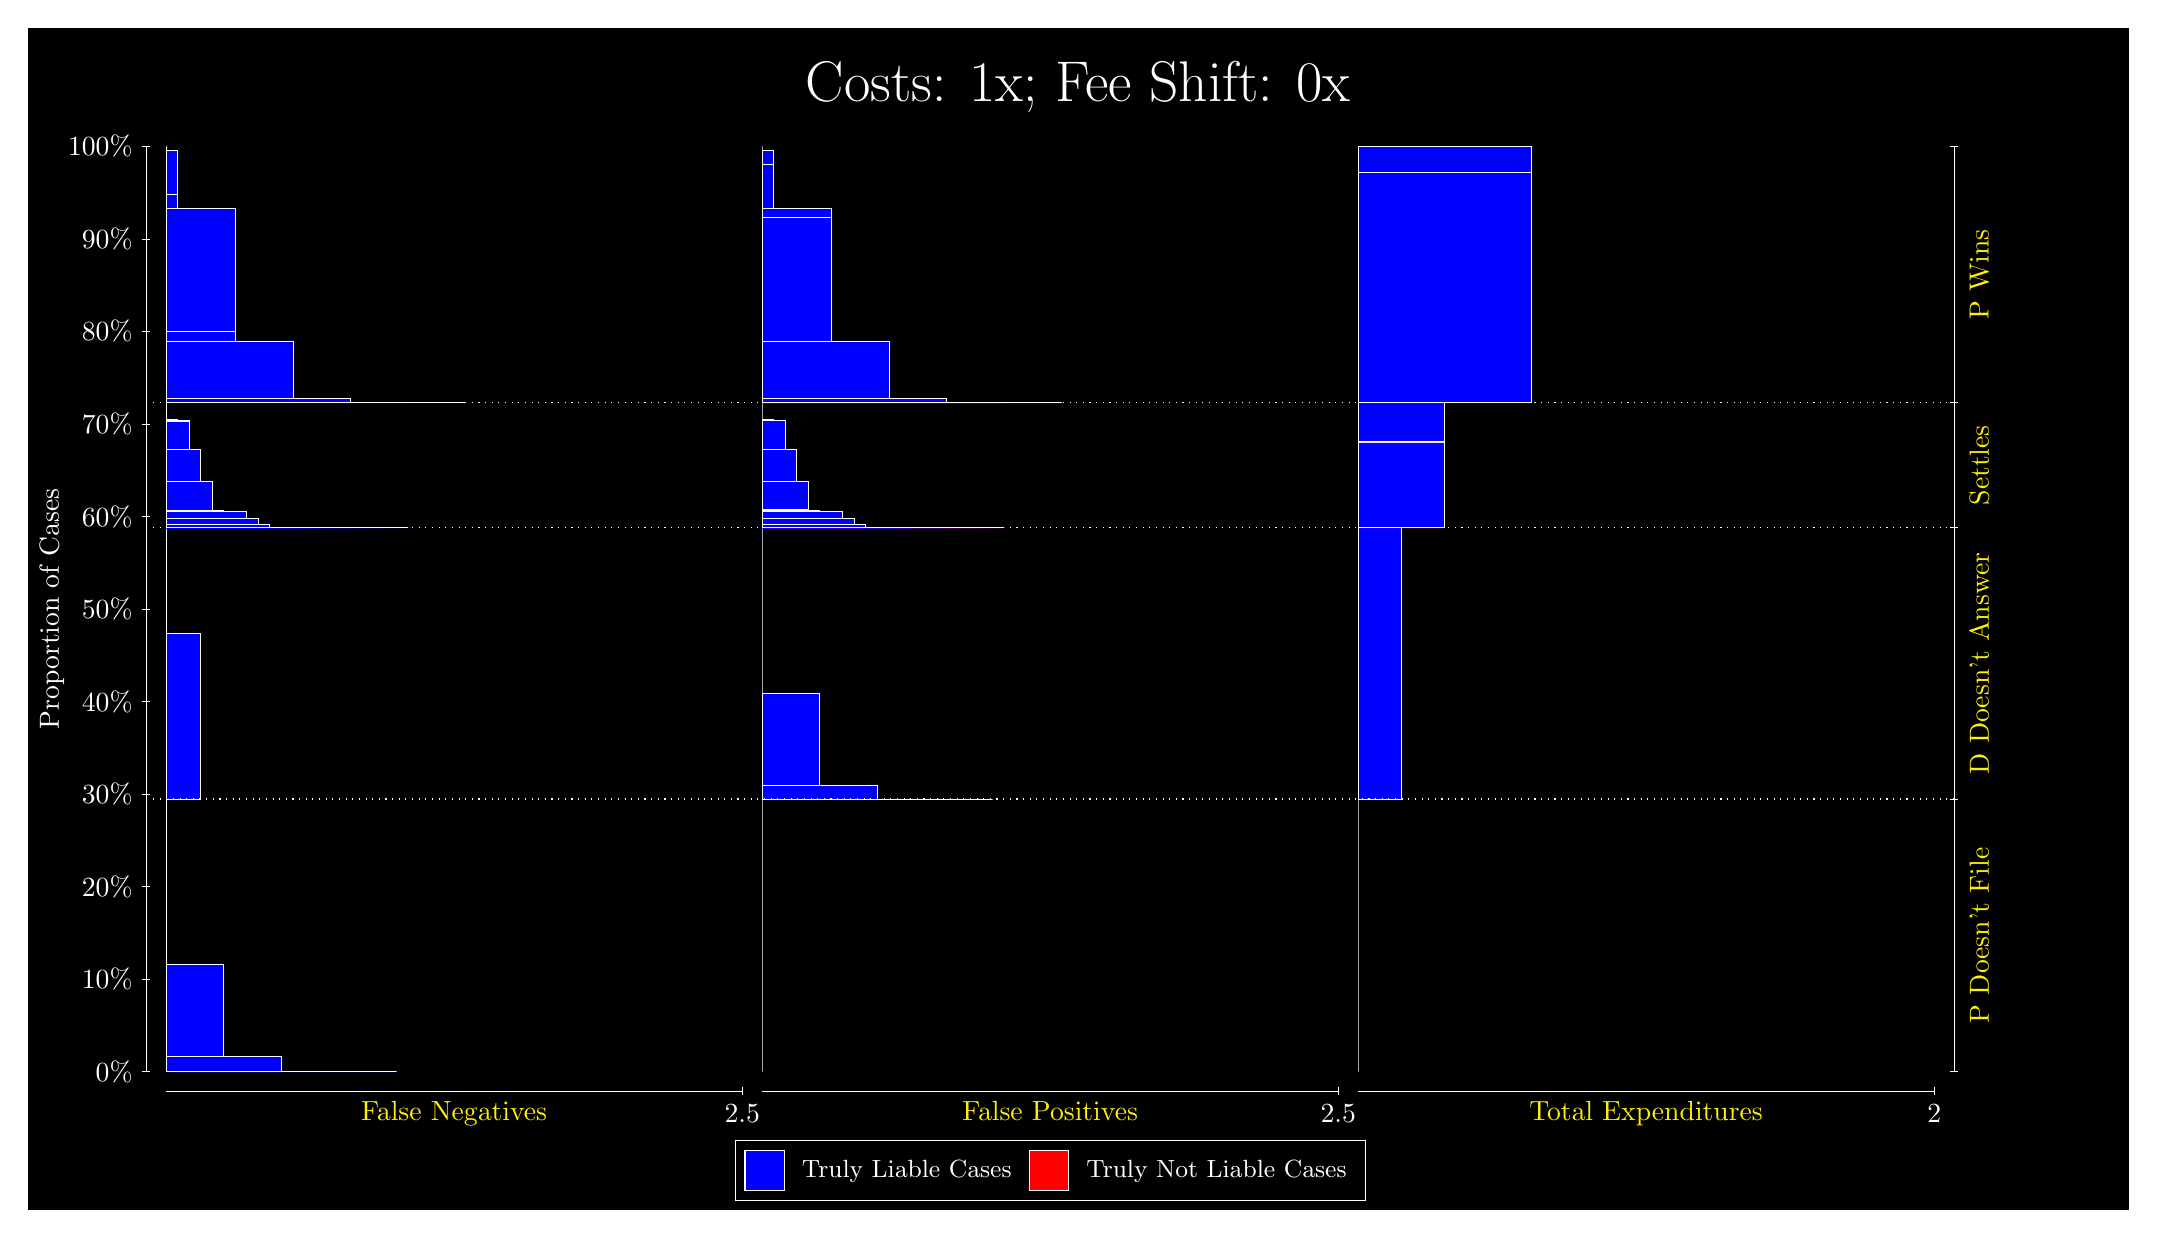
\begin{tikzpicture}
\draw[fill=black] (0,0) rectangle (26.667,15);
\draw[text=white] (0,13.5) rectangle (26.667,15) node[midway] {\huge Costs: 1x; Fee Shift: 0x};
\draw[white, very thin] (1.5,1.75) -- (1.5,13.5);
\node[rotate=90, text=white, anchor=center] at (0.3, 7.625) {Proportion of Cases};
\draw[white, very thin] (1.45,1.75) -- (1.55,1.75);
\node[text=white, anchor=east] at (1.45, 1.75) {0\%};
\draw[white, very thin] (1.45,2.925) -- (1.55,2.925);
\node[text=white, anchor=east] at (1.45, 2.925) {10\%};
\draw[white, very thin] (1.45,4.1) -- (1.55,4.1);
\node[text=white, anchor=east] at (1.45, 4.1) {20\%};
\draw[white, very thin] (1.45,5.275) -- (1.55,5.275);
\node[text=white, anchor=east] at (1.45, 5.275) {30\%};
\draw[white, very thin] (1.45,6.45) -- (1.55,6.45);
\node[text=white, anchor=east] at (1.45, 6.45) {40\%};
\draw[white, very thin] (1.45,7.625) -- (1.55,7.625);
\node[text=white, anchor=east] at (1.45, 7.625) {50\%};
\draw[white, very thin] (1.45,8.8) -- (1.55,8.8);
\node[text=white, anchor=east] at (1.45, 8.8) {60\%};
\draw[white, very thin] (1.45,9.975) -- (1.55,9.975);
\node[text=white, anchor=east] at (1.45, 9.975) {70\%};
\draw[white, very thin] (1.45,11.15) -- (1.55,11.15);
\node[text=white, anchor=east] at (1.45, 11.15) {80\%};
\draw[white, very thin] (1.45,12.325) -- (1.55,12.325);
\node[text=white, anchor=east] at (1.45, 12.325) {90\%};
\draw[white, very thin] (1.45,13.5) -- (1.55,13.5);
\node[text=white, anchor=east] at (1.45, 13.5) {100\%};

\draw[white, very thin] (24.457,1.75) -- (24.457,13.5);
\draw[white, very thin] (24.407,1.75) -- (24.507,1.75);
\node[anchor=west] at (24.407, 1.75) {};
\draw[white, very thin] (24.407,5.2117) -- (24.507,5.2117);
\node[anchor=west] at (24.407, 5.2117) {};
\draw[white, very thin] (24.407,8.6568) -- (24.507,8.6568);
\node[anchor=west] at (24.407, 8.6568) {};
\draw[white, very thin] (24.407,10.245) -- (24.507,10.245);
\node[anchor=west] at (24.407, 10.245) {};
\draw[white, very thin] (24.407,13.5) -- (24.507,13.5);
\node[anchor=west] at (24.407, 13.5) {};

\draw[white, very thin, fill=blue] (1.75,1.75) rectangle (4.6775,1.75);
\draw[white, very thin, fill=blue] (1.75,1.75) rectangle (3.9457,1.7516);
\draw[white, very thin, fill=blue] (1.75,1.7516) rectangle (3.2138,1.9396);
\draw[white, very thin, fill=blue] (1.75,1.9396) rectangle (2.4819,3.1085);
\draw[white, very thin, fill=red] (1.75,3.1085) rectangle (1.75,3.1085);
\draw[white, very thin, fill=blue] (1.75,3.1085) rectangle (1.75,5.2117);
\draw[white, very thin, fill=blue] (1.75,5.2117) rectangle (2.1891,7.3149);
\draw[white, very thin, fill=red] (1.75,7.3149) rectangle (1.75,7.3149);
\draw[white, very thin, fill=blue] (1.75,7.3149) rectangle (1.75,8.6568);
\draw[white, very thin, fill=blue] (1.75,8.6568) rectangle (4.8239,8.6568);
\draw[white, very thin, fill=blue] (1.75,8.6568) rectangle (4.5312,8.6568);
\draw[white, very thin, fill=blue] (1.75,8.6568) rectangle (4.2384,8.6568);
\draw[white, very thin, fill=blue] (1.75,8.6568) rectangle (4.092,8.6568);
\draw[white, very thin, fill=blue] (1.75,8.6568) rectangle (3.7993,8.6568);
\draw[white, very thin, fill=blue] (1.75,8.6568) rectangle (3.6529,8.657);
\draw[white, very thin, fill=blue] (1.75,8.657) rectangle (3.5065,8.6571);
\draw[white, very thin, fill=blue] (1.75,8.6571) rectangle (3.3602,8.6571);
\draw[white, very thin, fill=blue] (1.75,8.6571) rectangle (3.0674,8.7037);
\draw[white, very thin, fill=blue] (1.75,8.7037) rectangle (3.0674,8.7037);
\draw[white, very thin, fill=blue] (1.75,8.7037) rectangle (2.921,8.7822);
\draw[white, very thin, fill=blue] (1.75,8.7822) rectangle (2.7746,8.8698);
\draw[white, very thin, fill=blue] (1.75,8.8698) rectangle (2.6283,8.8703);
\draw[white, very thin, fill=blue] (1.75,8.8703) rectangle (2.4819,8.8837);
\draw[white, very thin, fill=blue] (1.75,8.8837) rectangle (2.3355,9.2398);
\draw[white, very thin, fill=blue] (1.75,9.2398) rectangle (2.3355,9.2439);
\draw[white, very thin, fill=blue] (1.75,9.2439) rectangle (2.1891,9.6584);
\draw[white, very thin, fill=blue] (1.75,9.6584) rectangle (2.0428,10.014);
\draw[white, very thin, fill=blue] (1.75,10.014) rectangle (2.0428,10.018);
\draw[white, very thin, fill=blue] (1.75,10.018) rectangle (1.8964,10.032);
\draw[white, very thin, fill=red] (1.75,10.032) rectangle (1.75,10.032);
\draw[white, very thin, fill=blue] (1.75,10.032) rectangle (1.75,10.245);
\draw[white, very thin, fill=blue] (1.75,10.245) rectangle (5.5558,10.245);
\draw[white, very thin, fill=blue] (1.75,10.245) rectangle (4.8239,10.245);
\draw[white, very thin, fill=blue] (1.75,10.245) rectangle (4.092,10.299);
\draw[white, very thin, fill=blue] (1.75,10.299) rectangle (3.3602,11.028);
\draw[white, very thin, fill=blue] (1.75,11.028) rectangle (2.6283,11.145);
\draw[white, very thin, fill=blue] (1.75,11.145) rectangle (2.6283,12.716);
\draw[white, very thin, fill=blue] (1.75,12.716) rectangle (1.8964,12.891);
\draw[white, very thin, fill=blue] (1.75,12.891) rectangle (1.8964,13.446);
\draw[white, very thin, fill=red] (1.75,13.446) rectangle (1.75,13.446);
\draw[white, very thin, fill=blue] (1.75,13.446) rectangle (1.75,13.5);
\draw[white, very thin, fill=red] (9.3189,1.75) rectangle (9.3189,1.75);
\draw[white, very thin, fill=blue] (9.3189,1.75) rectangle (9.3189,5.2117);
\draw[white, very thin, fill=red] (9.3189,5.2117) rectangle (12.246,5.2117);
\draw[white, very thin, fill=blue] (9.3189,5.2117) rectangle (12.246,5.2117);
\draw[white, very thin, fill=blue] (9.3189,5.2117) rectangle (11.515,5.2125);
\draw[white, very thin, fill=blue] (9.3189,5.2125) rectangle (10.783,5.3855);
\draw[white, very thin, fill=blue] (9.3189,5.3855) rectangle (10.051,6.5536);
\draw[white, very thin, fill=blue] (9.3189,6.5536) rectangle (9.3189,8.6568);
\draw[white, very thin, fill=red] (9.3189,8.6568) rectangle (12.393,8.6568);
\draw[white, very thin, fill=blue] (9.3189,8.6568) rectangle (12.393,8.6568);
\draw[white, very thin, fill=red] (9.3189,8.6568) rectangle (12.1,8.6568);
\draw[white, very thin, fill=blue] (9.3189,8.6568) rectangle (12.1,8.6568);
\draw[white, very thin, fill=red] (9.3189,8.6568) rectangle (11.807,8.6568);
\draw[white, very thin, fill=blue] (9.3189,8.6568) rectangle (11.807,8.6568);
\draw[white, very thin, fill=blue] (9.3189,8.6568) rectangle (11.661,8.6568);
\draw[white, very thin, fill=blue] (9.3189,8.6568) rectangle (11.368,8.6568);
\draw[white, very thin, fill=red] (9.3189,8.6568) rectangle (11.222,8.6568);
\draw[white, very thin, fill=blue] (9.3189,8.6568) rectangle (11.222,8.657);
\draw[white, very thin, fill=blue] (9.3189,8.657) rectangle (11.075,8.6571);
\draw[white, very thin, fill=blue] (9.3189,8.6571) rectangle (10.929,8.6571);
\draw[white, very thin, fill=blue] (9.3189,8.6571) rectangle (10.636,8.6571);
\draw[white, very thin, fill=red] (9.3189,8.6571) rectangle (10.636,8.6571);
\draw[white, very thin, fill=blue] (9.3189,8.6571) rectangle (10.636,8.7032);
\draw[white, very thin, fill=blue] (9.3189,8.7032) rectangle (10.49,8.7817);
\draw[white, very thin, fill=red] (9.3189,8.7817) rectangle (10.344,8.7817);
\draw[white, very thin, fill=blue] (9.3189,8.7817) rectangle (10.344,8.8692);
\draw[white, very thin, fill=blue] (9.3189,8.8692) rectangle (10.197,8.8697);
\draw[white, very thin, fill=red] (9.3189,8.8697) rectangle (10.051,8.8697);
\draw[white, very thin, fill=blue] (9.3189,8.8697) rectangle (10.051,8.8832);
\draw[white, very thin, fill=blue] (9.3189,8.8832) rectangle (9.9044,8.8872);
\draw[white, very thin, fill=blue] (9.3189,8.8872) rectangle (9.9044,9.243);
\draw[white, very thin, fill=blue] (9.3189,9.243) rectangle (9.758,9.6576);
\draw[white, very thin, fill=blue] (9.3189,9.6576) rectangle (9.6116,10.018);
\draw[white, very thin, fill=blue] (9.3189,10.018) rectangle (9.4652,10.031);
\draw[white, very thin, fill=blue] (9.3189,10.031) rectangle (9.3189,10.245);
\draw[white, very thin, fill=red] (9.3189,10.245) rectangle (13.125,10.245);
\draw[white, very thin, fill=blue] (9.3189,10.245) rectangle (13.125,10.245);
\draw[white, very thin, fill=red] (9.3189,10.245) rectangle (12.393,10.245);
\draw[white, very thin, fill=blue] (9.3189,10.245) rectangle (12.393,10.245);
\draw[white, very thin, fill=red] (9.3189,10.245) rectangle (11.661,10.245);
\draw[white, very thin, fill=blue] (9.3189,10.245) rectangle (11.661,10.299);
\draw[white, very thin, fill=red] (9.3189,10.299) rectangle (10.929,10.299);
\draw[white, very thin, fill=blue] (9.3189,10.299) rectangle (10.929,11.028);
\draw[white, very thin, fill=blue] (9.3189,11.028) rectangle (10.197,12.599);
\draw[white, very thin, fill=red] (9.3189,12.599) rectangle (10.197,12.599);
\draw[white, very thin, fill=blue] (9.3189,12.599) rectangle (10.197,12.717);
\draw[white, very thin, fill=blue] (9.3189,12.717) rectangle (9.4652,13.271);
\draw[white, very thin, fill=blue] (9.3189,13.271) rectangle (9.4652,13.446);
\draw[white, very thin, fill=blue] (9.3189,13.446) rectangle (9.3189,13.5);
\draw[white, very thin, fill=red] (16.888,1.75) rectangle (16.888,1.75);
\draw[white, very thin, fill=blue] (16.888,1.75) rectangle (16.888,5.2117);
\draw[white, very thin, fill=red] (16.888,5.2117) rectangle (17.437,5.2117);
\draw[white, very thin, fill=blue] (16.888,5.2117) rectangle (17.437,8.6568);
\draw[white, very thin, fill=red] (16.888,8.6568) rectangle (17.986,8.6568);
\draw[white, very thin, fill=blue] (16.888,8.6568) rectangle (17.986,9.7371);
\draw[white, very thin, fill=red] (16.888,9.7371) rectangle (17.986,9.7371);
\draw[white, very thin, fill=blue] (16.888,9.7371) rectangle (17.986,9.7511);
\draw[white, very thin, fill=red] (16.888,9.7511) rectangle (17.986,9.7511);
\draw[white, very thin, fill=blue] (16.888,9.7511) rectangle (17.986,10.245);
\draw[white, very thin, fill=red] (16.888,10.245) rectangle (19.083,10.245);
\draw[white, very thin, fill=blue] (16.888,10.245) rectangle (19.083,13.176);
\draw[white, very thin, fill=red] (16.888,13.176) rectangle (19.083,13.176);
\draw[white, very thin, fill=blue] (16.888,13.176) rectangle (19.083,13.5);
\draw[white, dotted] (1.5,5.2117) -- (24.457,5.2117);
\draw[white, dotted] (1.5,8.6568) -- (24.457,8.6568);
\draw[white, dotted] (1.5,10.245) -- (24.457,10.245);
\draw[white, very thin] (1.75,1.5) -- (9.0689,1.5);
\node[text=yellow, anchor=north] at (5.4094, 1.5) {False Negatives};
\draw[white, very thin] (9.0689,1.45) -- (9.0689,1.55);
\node[text=white, anchor=north] at (9.0689, 1.45) {2.5};

\draw[white, very thin] (9.3189,1.5) -- (16.638,1.5);
\node[text=yellow, anchor=north] at (12.978, 1.5) {False Positives};
\draw[white, very thin] (16.638,1.45) -- (16.638,1.55);
\node[text=white, anchor=north] at (16.638, 1.45) {2.5};

\draw[white, very thin] (16.888,1.5) -- (24.207,1.5);
\node[text=yellow, anchor=north] at (20.547, 1.5) {Total Expenditures};
\draw[white, very thin] (24.207,1.45) -- (24.207,1.55);
\node[text=white, anchor=north] at (24.207, 1.45) {2};

\node[text=yellow, centered, rotate=90] at (24.777, 3.4809) {P Doesn't File};
\node[text=yellow, centered, rotate=90] at (24.777, 6.9343) {D Doesn't Answer};
\node[text=yellow, centered, rotate=90] at (24.777, 9.4507) {Settles};
\node[text=yellow, centered, rotate=90] at (24.777, 11.872) {P Wins};

\draw (12.978300999999998,1.5) node[draw=none] (baseCoordinate) {};
\begin{scope}[align=center]
        \matrix[scale=0.5, draw=white, below=0.5cm of baseCoordinate, nodes={draw}, column sep=0.1cm]{
            \node[rectangle, draw, minimum width=0.5cm, minimum height=0.5cm, fill=blue] {}; &
            \node[draw=none, font=\small, text=white] (B) {Truly Liable Cases}; &
            \node[rectangle, draw, minimum width=0.5cm, minimum height=0.5cm, fill=red] {}; &
            \node[draw=none, font=\small, text=white] (B) {Truly Not Liable Cases}; \\
            };
\end{scope}

\end{tikzpicture}
\end{document}